\documentclass[border=10pt]{standalone}
\usepackage{pgfplots}
\pgfplotsset{compat=1.17}
\begin{document}
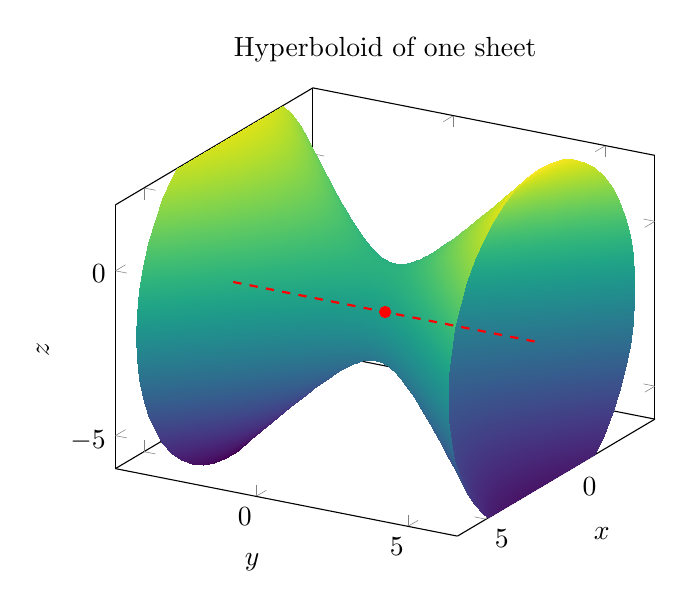
\begin{tikzpicture}
\begin{axis}[
    view={120}{20},
    xlabel=$x$,
    ylabel=$y$,
    zlabel=$z$,
    title={Hyperboloid of one sheet},
    xmin=-4,xmax=6,
    ymin=-4,ymax=6,
    zmin=-6,zmax=2,
    axis equal,
    colormap/viridis,
    samples=50,
    samples y=50,
    domain=-2:2,
    y domain=0:360,
]
\addplot3[surf,shader=interp,z buffer=sort]
({1+sqrt(2)*cosh(x)*cos(y)},
 {1+sqrt(2)*sinh(x)},
 {-2+sqrt(2)*cosh(x)*sin(y)});
\addplot3[red,thick,dashed] coordinates {(1,-4,-2) (1,6,-2)};
\addplot3[only marks,mark=*,red] coordinates {(1,1,-2)};
\end{axis}
\end{tikzpicture}
\end{document}
